90. По теореме Виета $x_1+x_2=a^2-5a=a(a-5)<0\Leftrightarrow a\in(0;5).$ Также необходимо проверить, что корни существуют, то есть $D\geqslant0,\ (a^2-5a)^2-4\cdot4a^2=(a^2-5a-4a)(a^2-5a+4a)=a(a-9)a(a-1)=a^2(a-9)(a-1)\geqslant0.$ Применив метод интервалов, найдём ответ:
\begin{figure}[ht!]
\center{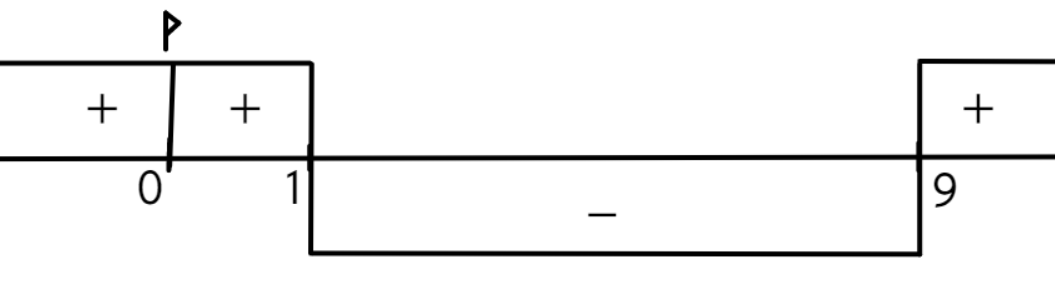
\includegraphics[scale=0.35]{isl90.png}}
\end{figure}
$a\in[-\infty;1]\cup[9;+\infty).$\\ Окончательным ответом в задаче будет пересечение полученных ответов, $a\in (0;1].$\\
